\documentclass[12pt, titlepage]{caesar_book}
\usepackage{amssymb, amsmath, hyperref,setspace,physics}
\usepackage{color,parskip,siunitx}
\usepackage{epsfig, graphicx, todonotes,sidenotes}
\usepackage{verbatim}

\begin{document}
I need to decide what to focus on in this work. There is a lot of information out there about the laser, different regimes. Do I fully derive the cold-fluid plasma equations
\section{Cold Fluid Equations}

In treating a plasma mathematically as a fluid, we must consider that the fluid particles
will also have to obey the Maxwell equations. This means that the well known Navier-Stokes
equation has to be modified to include additional terms. In a simple model, where the electron
motion is confined to motion in the $x$ direction, and $T=0$ and $B=0$, the full equations
needed to describe the cold plasma is given by:
\begin{subequations}
    \begin{align}
        \div{\vb{E}} & = 4 \pi e \qty(n_i-n_e) \\
    m n_e \left( \pdv{\vb{v}_e}{t} \right) &= -e n_e \vb{E} \\
        \pdv{n_e}{t} + \div{ \qty(n_e \vb{v}_e)} & = 0\\
    \end{align}
\end{subequations}

With an small incident electric field, we can linearize the equations about
equationbrium:
\begin{align*}
    &\vb{E} \rightarrow \vb{E_0} + \vb{E_1}\\
    &n \rightarrow 0 + \delta n \\
    &\vb{v} \rightarrow \vb{v_0} + \vb{v_1}
\end{align*}

Only keeping terms to first order, and assuming that the perturbations vary sinusoidally,
this gives us the disperion of Langumir waves in a cold plasma. 

\begin{equation}
\label{eq:dispersion}
\omega = \qty(\frac{ne^2}{m_e \epsilon})^{1/2} = \omega_p,
\end{equation}
with $e$ as the electron's charge, $m_e$ the electron's mass, $n$ is the number
density of electrons in the medium, and $\epsilon$ is the permativity of the plasma.

\section{Laser-Driven Plasma Waves for Particle Acceleration and X-Ray Production}
The nonlinear case is where $a_0 = e\vb{A}(m_e c^2)^{-1} > 1$. Transfering to
a frame moving at the same rate as the phase veloctiy of the packet,  $t\rightarrow \tau$, $z-v_g t \rightarrow \xi $, and assuming that the pulse 
doesn't evolve, we can get Poisson's equation:
\begin{equation}
    \pdv[2]{\phi}{\tau} = k_p^2 \qty( \frac{n_e}{n_{e0}} - 1)
\end{equation}
        \todo{still need to be able to derive this \ldots}
The relativisitic factor then becomes:
\begin{equation}
    \gamma = \frac{\gamma_\bot^2}{1-\beta_z^2} 
\end{equation}
I think I may just show a figure for the non-linear case. The equation is hard 
to look at and understand. Cite heavily.
\section{Trapping Electrons}
In order to be accelerated by the co-propogating electric field created by the plasmon, the electrons need to be travelling at some minimum speed. In the plasmon frame of reference, what an electron will see is, roughly, an ion-sphere. If we confine the electrons motion to 1D, then it can exhibit periodic motion about the centre of this sphere. 

However, for this to work, the electron needs to have some minimum energy. Imagining a simple harmonic potential that is moving at some brisk speed $v_b > \sqrt{2 V_\mathrm{height of well}/m} $, we can see that an electron at rest will not be trapped: transforming to the potentials frame of reference, the electron will have too much energy to be trapped.
\begin{marginfigure}
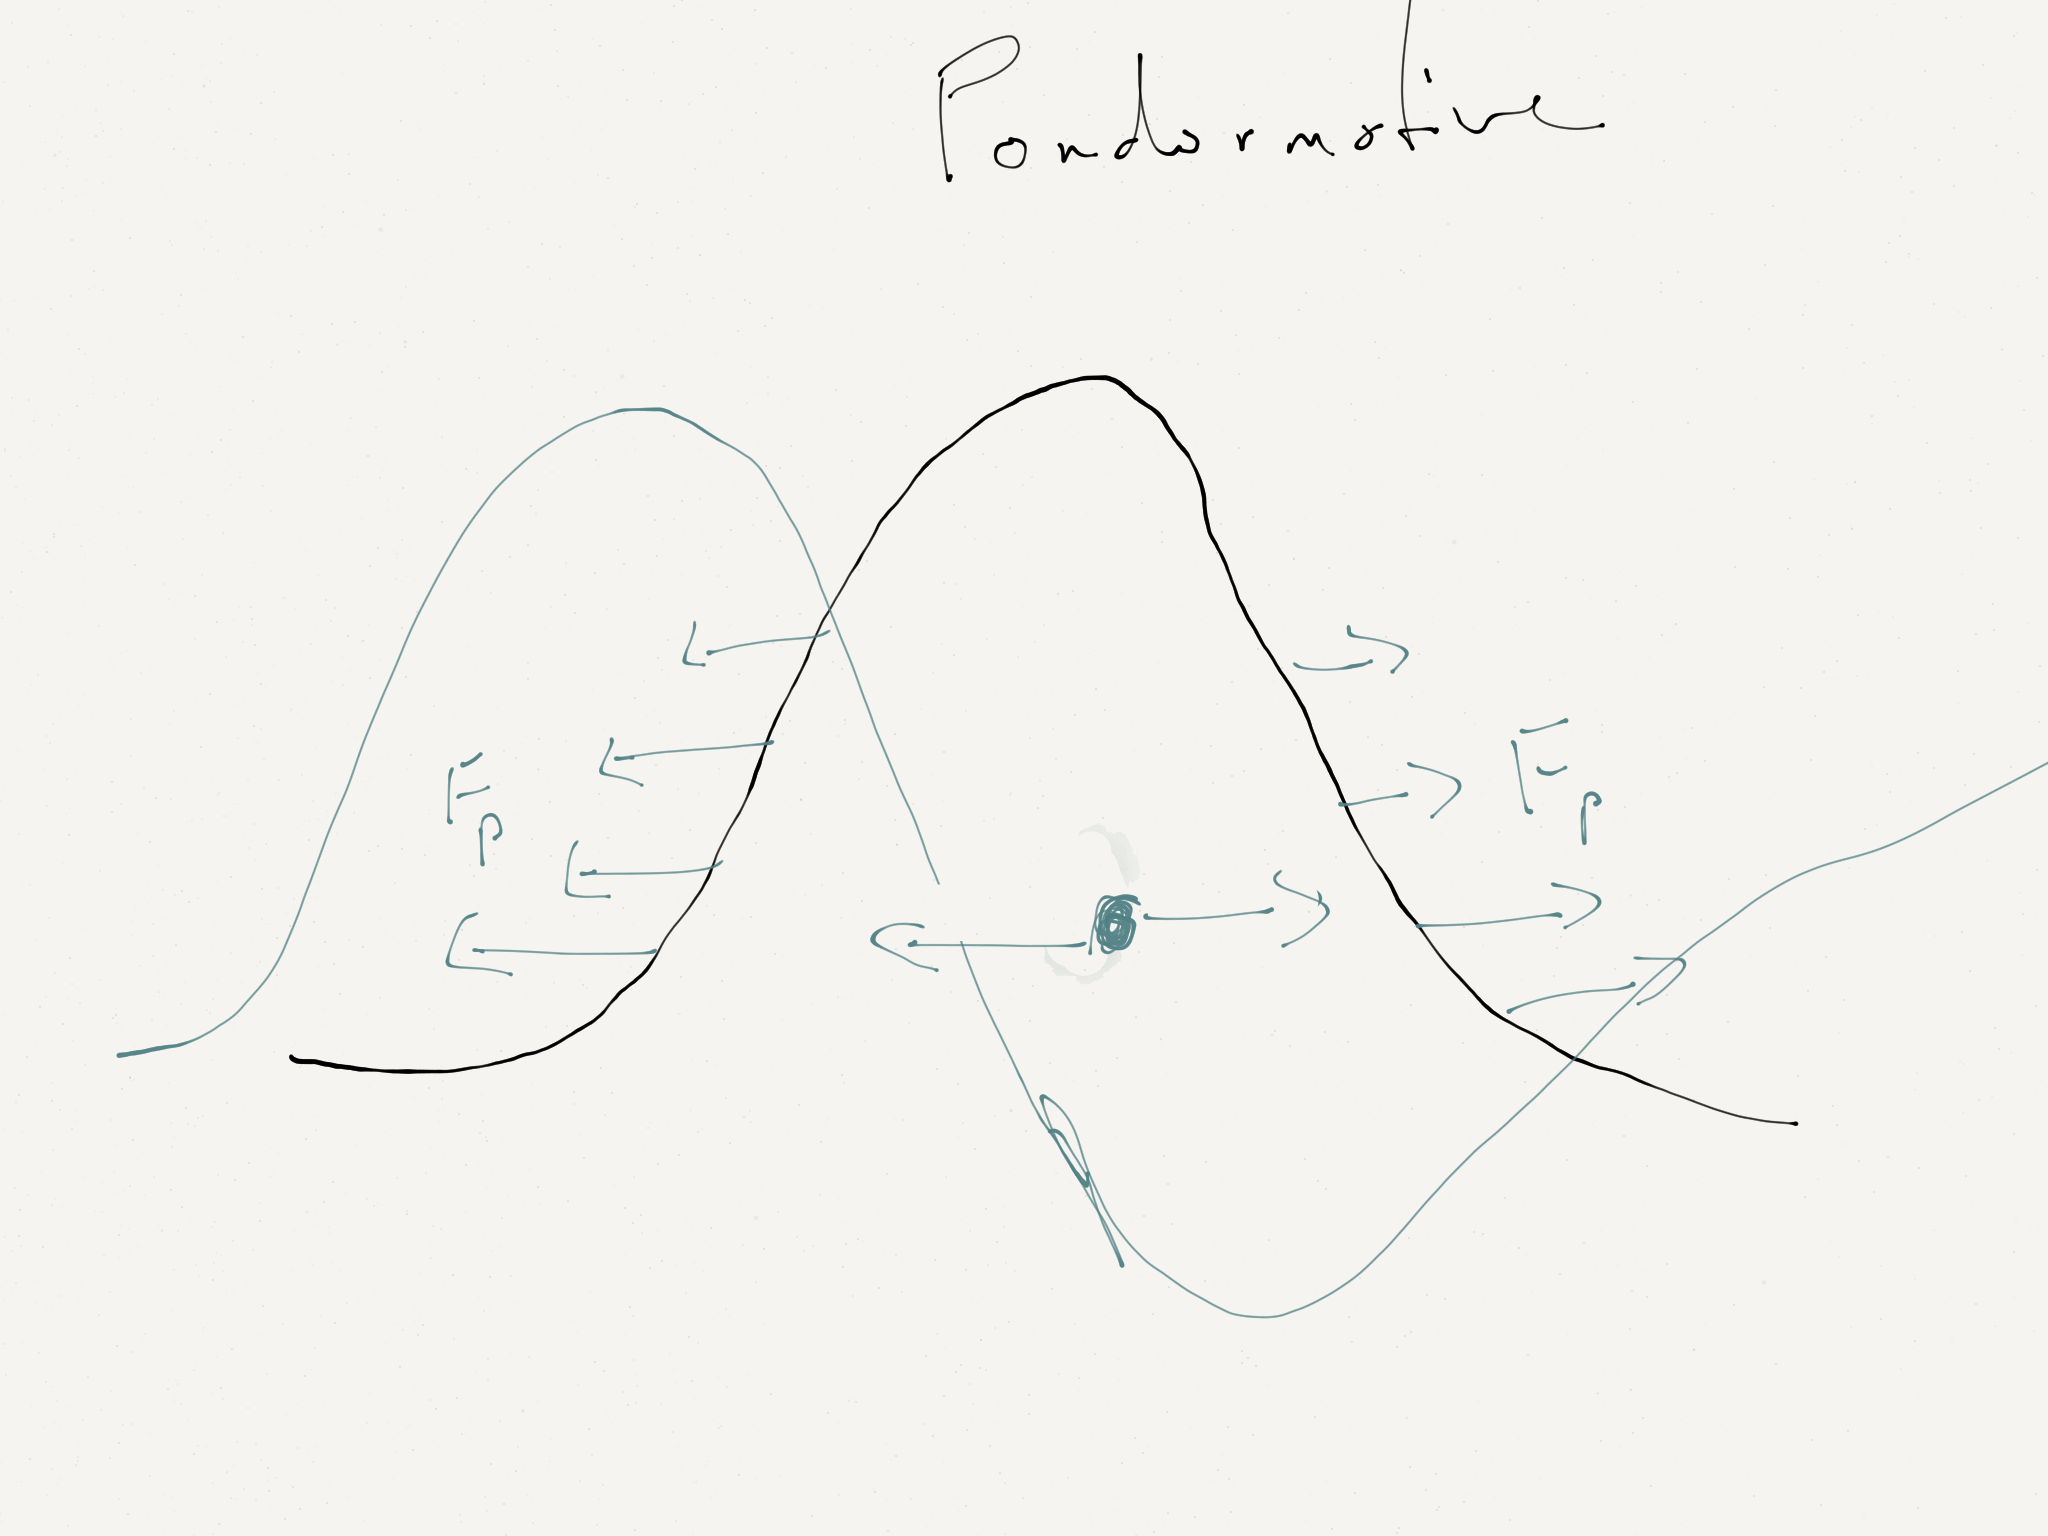
\includegraphics[width=4cm]{./pf.png}
\caption{This shows the ponderomotive force. It will expel electrons from the laser
packet region, in effect creating an ion-sphere that will create an accelerating force
on a 'test' electron}
\end{marginfigure}
This is quite similar to the case we are describing: however, we now have to consider that the electron's motion is going to be relativistic. In this case, the minimum energy an electron needs is given by \todo{need to add citation}:
\begin{equation}
\gamma_\mathrm{min} = \Delta \phi / (1+\beta_p) + \beta_p/(2 \Delta \phi)
\end{equation}

\todo{I'm not sure about adding this equation in. Probably take it out-- leave it at a general discussion and maybe show a plot of what a test electron's trajectory would look like.}

For a very specific value of the accelerating electric field the background electrons that make up the density flucuations will actually meet the requirements to be trapped in this way. This gives rise to the phenomena of wavebreaking. In contrast to the perhaps more familiar example of water-wave's breaking, plasma wavebreaking is not a dispersion related phenomena. It is a non-linear effect, where the accelerating field created by the density flucuations of electrons in the plasma is strong enough to directly effect the density flucuations themselves.

Wavebreaking is a useful phenomena for LWFA as it creates a larger field that can give more energy to the electrons. The phenomelogical differences between a linear plasmon and a wavebroken plasmon are show in Figure \todo{add figure}.

{\em Trapping and accleration in nonlinear plasma waves was very useful-- a little terse. Mainly, they just guessed the hamiltonian for the system, plotted traj. around the fixed points and then said that the largest energy gain is by largest traj in phase space. (makes sense). Then they solve for the minimun kinetic energy a test electron would have on the largest traj. This then is the minimum energy required for an electron to be caught. I'm still not quite sure about some of the sublties about the phase (position) relationship to the energy.}

\section{Laboratory Visualization of Laser-Driven Plasma Accelerators in the BUbble Regime}
\section{Injection in Plasma-Based Electron Accelerators}
\section{Experimental Programs}
\section{Texas}
Should include figure from the Texas people. 

Using chirped-pulse-amplification (CPA), extremely high peak power can be achieved by modern ultra-fast laser. CPA works by first creating an ultrashort

in time. Once the pulse has been stretched out, the peak power will decrease, and the pulse can be safely sent through a laser-amplification stage, typically with a gain between 2-100 per pass. Once the pulse has been safely amplified, it can be re-compressed, using a technology such as parallel grating compressor.
The whole process can increase the peak power from $\SIrange{e3}{e14}{\watt}$, as
in the Texas PetaWatt Laser at UT-Austin.

With laser peak power this high, it can easily ionize a solid target-- creating
the plasma that it will be propogating through. In the Texas setup, the laser pulse is incident on a gas-cell, where it will create the co-propogating density wave by `blowing out' the electrons from the region of the laser pulse.

This will set-up the longitudinal electric field that acts to accelerate the electrons. The electrons will be accelerated for the duration of the glass cell, and then be expelled into free space.  
There is an array of sensors to measure the incoming electrons. First, they pass
through a magnetic field, which bends them with a radius of curvature $ r = mv/(eB)$ \todo{make this relativisitic}. The slower moving electrons will be bent more, hitting an imagining plate. The faster moving electrons will continue on, largely undeflected. They are incident on two imagining plates: the first is a high-sensitivity plate that picks up medium energy electrons ($E >\SI{0.5}{\giga\electronvolt}$) that have been energery dispersed (not well collumate), the
second imagining plate is the one that picks up the well-collumated electron beam at $E \approx \SI{2}{\giga\electronvolt}$. Additionally, tungsten posts are placed at various places downsteam of the exit aperature. These posts will
cast shadows on the imaged plates, and simple geometry can be used to reveal
the trajectory of the electron beam.

\section{SLAC}

\section{Europe}

\section{Future Work}

The initial results in 2004 by [][][] where very promising, and progress is being made at an accelerated rate. However, it is still difficult to understand the minutia of the dynamics of LPA. This is due to the highly non-linear nature of the process. To make further progress, advances need to be made in three catagories: first, finer control over the laser parameters needs to be established, the pulse duration, pulse shape, pulse energy; second, better imaging and
diagnostic technologies need to be developed so that the pulse can be imaged in situ; third, more work needs to be done on the theoretical side so that experimentalists have an idea of what knobs to twist.
\end{document}
